% !TeX spellcheck = <none>
\documentclass{article}
\usepackage{graphicx}
\usepackage[italian]{babel}
\usepackage[latin1]{inputenc}
\usepackage{lipsum}% http://ctan.org/pkg/lipsum
\begin{document}
	\title{Linear discriminant analisys con CUDA C}
	\author{Francesco~Polvere
		\thanks{F. Polvere, Corso di GPU computing,  A/A 2017-2018, Universit\'a degli studi di Milano,
			via Celoria 28, Milano, Italia \protect\\
			% note need leading \protect in front of \\ to get a newline within \thanks as
			% \\ is fragile and will error, could use \hfil\break instead.
			E-mail: francesco.polvere@studenti.unimi.it}%
	}
	\maketitle
	\begin{abstract}
		%\boldmath
		In questo documento viene presentata una implementazione dell'algoritmo di linear discriminant analisys tramite l'utilizzo della GPU sulla piattaforma CUDA. 
		L'implementazione parallela viene confrontata con l'implementazione classica in C, tramite la misura di tempo di esecuzione e colcolatone lo speed-up.
	
	
\end{abstract}
\section{Introduzione}
Da una analisi del metodo di LDA, si pu� notare la presenza di numerose operazioni su matrici che presentano un alto grado di parallelizzabilit�.
\section{Analisi dello stato dell'arte}
\lipsum[1-1]
\section{Modello teorico}
LDA � un metodo utilizzato per trovare una combinazione lineare di features che caratterizzato o separano due o pi� classi di oggetti o eventi. Il combinazione risultante pu� essere utilizzata  come classificatore lineare o ancor prima della classificazione, come operazione di riduzione di dimensionalit�.
\subsection{LDA Multiclasse}
Supponiamo di avere \(n\) classi. La Within-scatter matrix � calcolata come:

\[Sw = \sum_{i=1}^{C}\sum_{x app Ci }(x-x_{i})(x-x_{i})'\]

Mentre la between-scatter matrix � calcolata come:
\[Sb = \sum_{i=1}^{n}m_{i}(\overline{x}_{i}-\overline{x})(\overline{x}_{i}-\overline{x})'\]

Dove \(\overline{x}\) \'e la media totale di tutte le classi, \(m_{i}\) \'e il numero di dati di training per ogni classe.\\
Dopo aver ottenuto \(Sb\) e \(Sw\), vogliamo trovare l'equazione lineare che massimizza l'equazione in figura.

\[J(W) = \frac{|W^{T} S_{b}  W|}{|W^{T} S_{w} W|}\]

Si pu� dimostrare che la trasformazione W pu� essere ottenuta risolvendo un problema sugli autovalori:
\[S_{b}W = \lambda S_{w}W\]

\subsection{Parallelizzazione di LDA utilizzando CUDA}
Il dataset utilizzato � diviso in tre file, uno per ogni classe, contenente le osservazioni per ognuna di esse. Una volta caricati in memoria host, vengono copiati sulla sulla memoria device, in particolare nella global memory, il cui spazio � rilasciato solo al termine dell'esecuzione dell'intero programma.\\
L'allocazione su host � di tipo \textit{pinned} per permettere l'esecuzione sovrapposta del caricamento da host a device di ogni classe ed il calcolo della media della classe stessa.\\

\paragraph{Assunzioni e notazioni}
Si assume che i dati siano stati estratti da una distribuzione gaussiana.\\
Il numero di osservazioni � uguale per ogni classe.\\
\begin{itemize}
	\item C: numero di classi (o matrici)
	\item N: numero di osservazioni (o righe della matrice)
	\item M: numero di feature (o colonne della matrice)
\end{itemize}

\paragraph{Media della i-esima classe}
Per ogni classe vengono eseguite una \textit{cudaMemcpyAsync} per portare i dati sulla global memory del device ed il kernel che calcola ne la media (figura \ref{fig:means}).\\
I risultati sono mantenuti in global memory e non riportati in memoria host per ottimizzarne le prestazioni.\\
\begin{figure}[h]
	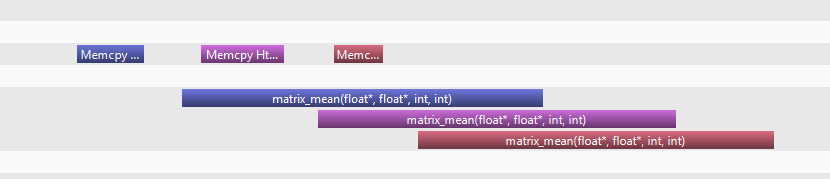
\includegraphics[width=\linewidth]{images/overlap_calcolo_media.PNG}
	\caption{Gli stream per il calcolo della media}
	\label{fig:means}
\end{figure}

\paragraph{Media totale}
La media totale � calcolata con un kernel (...) che esegue la somma degli C-vettori risultati dal calcolo precedente e dividendo per uno scalare che � il numero di classi.\\
Questi n-vettori avranno hanno dimensione
\paragraph{Between-scatter matrix}
Il calcolo della Between-scatter matrix necessit� di tre piccoli kernel.\\
Il kernel \textit{diff\_vect} si occupa di calcolare la differenza tra due vettori di dimensione \textit{M}, nel caso specifico tra il vettore media locale i-esimo e media globale. Successivamente si utilizza il kernel \textit{vector\_prod} per il calcolo del prodotto tra il vettore in uscita dal kernel precedente e la sua trasposta. Il risultato � una matrice quadrata di dimensione \textit{M X M}.\\
L'ultimo punto � la somma di tutte le C matrici in uscita dal kernel precedente.\\
Tutte e tre le operazioni sono eseguite da tutte le classi in stream diversi per ogni classe per permettere un livello di esecuzione concorrente maggiore.
\paragraph{Within-scatter matrix}
Il calcolo della Within-scatter matrix
\section{Simulazione ed esperimenti}
Sono stati sviluppati due algoritmi. Quello sequenziale e quello parallelo.
\subsection{Dataset}
Per il benchmark \'e stato utilizzato il dataset Iris, introdotto da Ronald Fisher. Il dataset consiste in tre classi, ognuna delle quali rappresenta una specie di pianta, con un numero di istanze di 50 per ogni classe, per un totale di 150 istanze.
Le variabili considerate sono quattro e consistono nella lunghezza e larghezza del sepalo e del petalo.
\section{Risultati ottenuti}
Il software � stato eseguito su un computer con le seguenti caratteristiche:
\begin{itemize}
	\item GPU: NVIDIA GeForce 610M, compute capability  2.1, architettura FERMI (2.1) con 48 Cores/SM.
	\item CPU: Intel(R) Core(TM) i7-3630QM CPU @ 2.40GHz, 2401 Mhz, 4 core, 8 processori logici
\end{itemize}

\paragraph{Grafici}
 



\section{Conclusioni}
\lipsum[1-2]
\end{document}